%%=============================================================================
%% Methodologie
%%=============================================================================

\chapter{\IfLanguageName{dutch}{Methodologie}{Methodology}}
\label{ch:methodologie}
In dit deel wordt eerst overlopen aan welke voorwaarden software moet voldoen om te kunnen dienen als leermiddel. Vervolgens worden deze voorwaarden afgetoetst aan de gevonden software om zoo een aantal test omgevingen voor te definiëren. Hierna woorden de resultaten van de tests besproken om af te sluiten met algemeen resultaat.

%% Hoe ben je te werk gegaan? Verdeel je onderzoek in grote fasen, en
%% licht in elke fase toe welke stappen je gevolgd hebt. Verantwoord waarom je
%% op deze manier te werk gegaan bent. Je moet kunnen aantonen dat je de best
%% mogelijke manier toegepast hebt om een antwoord te vinden op de
%% onderzoeksvraag.

\section{Selectie software}
Om software te vinden die toepasbaar is om gebruikt te worden als lesmateriaal moeten er bepaalde vereisten voldaan zijn.

\begin{itemize}
    \item Kosteloos zijn; als er kosten zijn mogen deze de leer ervaring niet ten nadele komen.
    \item Uitvoerbaar op de computers van de studenten. Mag door de verschillen in besturingssystemen van studenten computers niet te veel verschillen in werking.
    \item De software moet op zichzelf of in combinatie met ander software de volledige levenscyclus van containers kunnen tonen en niet te restrictief in gebruik zijn.
    \item Niet te complex zijn om te gebruiken.
    \item Geen verwaarloosde software zijn.
\end{itemize}
    
\subsection{Algemene toepassing voorwaarden op gevonden software}
Door een klassieke VM te gebruiken om daarin te werken kunnen de problemen met de uitvoerbaarheid op het gast besturingssystemen vermeden worden en zal de ingebruikname ook binnen de VM voor alle studenten hetzelfde zijn. Dit heeft ook het voordeel dat het besturingssysteem van de VM een Linux distributie kan zijn, een voorwaarde die nodig is om veel van software te kunnen draaien. De rest van deze sectie zal iets specifieker de gevonden technologieën overlopen.

Met uitzondering van technologieën die op Cloud berusten, de repositories of volledige Cloud services, zijn alle van de gevonden technologieën gratis te gebruiken. Ook is er door het OCI een zekere mate van mudulariteit tussen de technologieën. Software mag dan zelf niet de volledige orchestration kunnen doen, zal er een zekere integratie zijn met software dit dat wel kan.

\subsection{Engines en runtimes}
Qua geschiktheid om als runtime komen Docker engine en Podman het beste uit. Docker Dankzij zijn populariteit en veelvuldigheid. Hiermee is er ook veel onlinehulp te vinden voor het gebruik van Docker. Podman ’s vriendelijkheid als leermiddel is deels te danken doordat het zich opstelt als een duidelijk alternatief voor Docker op Linux distributies. De directe hulp een uitleg om met Podman te werken mag dan al iets minder zijn, die werking van Podman zou kort beschreven kunnen worden als hetzelfde als dat van Docker qua commando’s met een ingebouwde ondersteuning voor pods van meerdere containers.  Verder zou Containerd ook nog een alternatief kunnen zijn maar dan nipt op de rand van de complexiteit, zeker in vergelijking met Podman en Docker.

Om zelf te werken met Linux containers is te complex om een goede introductie tot containers te zijn. Windows containers zijn enkel mogelijk op bepaalde distributie van Windows en berusten verder op de Docker engine voor de uitvoering, hierdoor is de extra stap om met deze containers te werken ten opzichte van Docker geen meerwaarde als inleiding. Een gebrek aan uitleg voor het gebruik van cri-o doet twijfelen aan de geschiktheid voor Cri-o als runtime.  Het unieke verkooppunt van Kata containers, de mogelijkheid om ook VM’s als containers te draaien is een stap in complexiteit te ver om een goede inleiding to container virtualisatie te zijn.  De rest van de gevonden runtimes zijn te klein of al te lang zonder ondersteuning om met zekerheid te kunnen zeggen dat ze relevant zullen blijven voor containers en verwante technologieën.

\subsection{Orchestration}
Docker compose is een uitbreiding van de Docker engine en is daarmee ook gratis en heeft dezelfde vereisten als Docker, het wordt zelf standaard geïnstalleerd met de Docker desktop applicatie. Kubernetes en Nomad zijn verder nog twee softwarepakketten die goed zouden kunnen zijn om met te leren. Kubernetes is de meest gebruikte orchestration software en is daarmee zoals Docker voorzien van veel online tutorial. Het is open source en kan met veel van de runtimes werken. Voor het leren werken met Kubernetes is er ook Minikube die je lokaal in staat stel met Kubernetes te werken. Nomad is orchestration software die lijkt op Kubernetes maar toch zichzelf wilt onderscheiden van Kubernetes door meer dan alleen containers te kunnen beheren. 

De specifieke besturingen systemen orchestration DC/OS en Apache Mesos zijn te gelimiteerd tot het besturingssysteem en verder ook te complex om een duidelijke introductie te zijn tot container virtualisatie.  Openshift is een te commercieel en bedrijfsgericht product om makkelijk in gebruikt e worden genomen. En tenslotte is er nog de Docker swarm die zelf aan populariteit verliest ten opzichte van Kubernetes als software voor orchestration.


\subsection{Image repositories}
Met dat het OCI en hun container image geslaagd is in de standaardisatie container images zijn repositories vrij met elkaar te verwisselen. De Docker hub en de GitHub container registry zijn de meest geschikt om door een student als image repository te gebruiken.  Docker hub doordat het bijna overal als standaard gebruikt wordt en de GitHub omdat een student wellicht al een GitHub account hebben. Ook de kostenstructuur van de twee is te vergelijken met gratis publieke images en betaling vanaf een bepaalde drempel voor private images. Tijden het schrijven van deze thesis is de GitHub container registry wel no in een bètafase waardoor het volledig gebruik gratis is.

\subsection{Cloud hosting en servces}
Cloud hosting services kunnen een optie zijn maar afhankelijk van de host kan het dat een free trial niet toegang geeft tot alle tools die nodig zijn of is het moeilijk om gratis krediet te krijgen. Zo geeft Amazon geen gratis krediet meer of vraagt Google voor een creditcard.  Verder zal het maken van een image eerst lokaal moeten gebeuren waarvoor een lokale runtime nodig is. Hierdoor kan er even goed in eerste instantie lokaal verder gewerkt worden.

\section{Software Tests}
Wegens de modulariteit gecreëerd door het OCI zullen eerst de runtimes uitgeprobeerd worden om daarna te kijken naar de mogelijkheden van de runtimes om te werken met toegewijde orchestration software.

\subsection{Runtimes}
Voor deze is het voornaamste belang dat containers kunne gemaakt gedraaid en gestopt worden door middel van de runtime ook moet het persisteren van data naar een volume en het pullen van een image mogelijk zijn.

\paragraph{Docker Desktop}
De Docker desktop een applicatie voor Windows en Mac die Dockers engine combineert met Docker-compose, lokale Kubernetes, een dashboard en een eenvoudige verbinding met de Docker hub. Wegens de volledigheid van deze bundel zal dit als eerste uitgeprobeerd worden. Doordat de desktop applicatie niet voor Linux bestaat is deze echter niet volledig toepasbaar voor alle studenten. Een Linux gebruiker zou de delen apart moeten installeren. Dit is ook de software die direct op een laptop zal worden uitgevoerd en niet in een VM. Ook zal ik dit gebruiken als een baseline voor vergelijkingen. 

\paragraph{Fedora Podman}
Een eerste VM waarin ik het meest beloftevolle alternatief wil testen is Fedora workstation instantie. Deels omdat Fedora al gebruikt wordt tijdens het vak besturingssystemen en omdat het ook standaard met een Firefox webbrowser komt waarmee het gemakkelijk is om te testen of een webservice gebaseerde container draait.

\paragraph{Ubuntu Podman}
Om Podman ook uit te proberen op een ander besturingssysteem dan Fedora zal ook eens geprobeerd worden of dat het lukt om Podman te installeren op een Ubuntu distributie.

\subsection{Orchestration}
Voor orchestration moet het mogelijk zijn om een job of taak op basis van containers te maken, aan te passen en te stoppen. En ook om iets complexer dan een enkele container service te draaien.

\paragraph{Kubernetes gebundeld met Docker desktop}
De Docker desktop applicatie komt met de mogelijkheid om een lokale Kubernetes instantie te starten. Het lijkt dus interessant om Deze ook eens te testen.

\paragraph{Podman met Minikube voor Kubernetes}
Om te testen of dat het ook mogelijk is om met Podman als runtime te werken voor Kubernetes zal er ook geprobeerd worden om een Minikube instantie werkende met Podman op te zetten en gebruiken.

\paragraph{Docker engine en Nomad}
In tegenstelling tot Kubernetes en Minikube die meer vrijheid heeft voor de achterliggende runtime heeft Nomad op dit moment enkel ondersteuning voor de Docker engine om mee te werken voor het draaien van een containers. Dus voor het uitproberen van Nomad moet er met een Docker engine gewerkt worden.

\section{Resultaten software Tests}
In dit deel worden de resultaten en ondervindingen van het werken met de eerder opgestelde software test scenario’s overlopen. 

\subsection{Docker Desktop}
Het eerste dat uitgeprobeerd werd is de Docker desktop geïnstalleerd als applicatie op een laptop met 8 GB ram geheugen.

\paragraph{Installatie en set-up}
Het werken met Docker desktop direct geïnstalleerd op een Windows systeem moet er eerst het Windows Subsysteem voor Linux ingeschakeld worden. Docker verwijst hiervoor naar de help pagina’s van Microsoft. Omdat ik niet deel been van het Windows insiders program heb ik gewoon de manuele instructies van Microsoft \footnote{\url{https://docs.microsoft.com/en-us/windows/wsl/install-win10}} gevolgd om tot en met het opzetten van WSL2 als default uit te voeren. Het enigste dat hier wat specifieke aandacht vereist ten opzichte van de beschreven stappen is het controleren of dat de Windows versie geschikt is voor WSL.

Hierna werd de installer van Docker desktop uitvoeren, dit heeft een optie om WSL voor de gebruiker voor te bereiden maar omdat dit reeds gedaan heb ik niet kunnen testen of dat dit het volledig ennablen van WSL doet of enkel verantwoordelijk is voor het instellen van een Linux distributie in WSL waarmee de containers zullen worden uitgevoerd.

\paragraph{Ingebruikname}
Bij het eerste keer opstarten van de desktop applicatie staart het et een korte tutorial die enkel het pullen builden en uitvoeren van een eenvoudige container behandelt,  dit deels op een zeer korte introductie te zijn en te testen of dat de installatie gelukt is. Eveneens is het opstarten van de desktop applicatie de trigger om de backend die alles effectief draait ook te starten.

Vervolgens werd een uitgebreide tutorial van Docker gevolgd\footnote{\url{https://docs.docker.com/get-started/02_our_app/}}. Deze legde het werken met Docker en Docker compose zorgvuldig uit. Beginnende met een git repository die je zelf moet clonen om daarvan aan de hand van een Dockerfile een image te bouwen. Vervolgens deze image eens lokaal draaien, updaten en pushen naar de Docker hub. De Docker desktop applicatie werd ook gehanteerd om te demonstreren dat je deze dashboard ook je containers kan starten stoppen, pushen of verwijderen. De gepushte image kon vervolgens op een Play with Docker omgeving eens worden uitgevoerd om de overdraagbaarheid te demonstreren. Het werken met volumes voor het persisteren van data werd ook behandelt. 

\begin{figure}[h]
    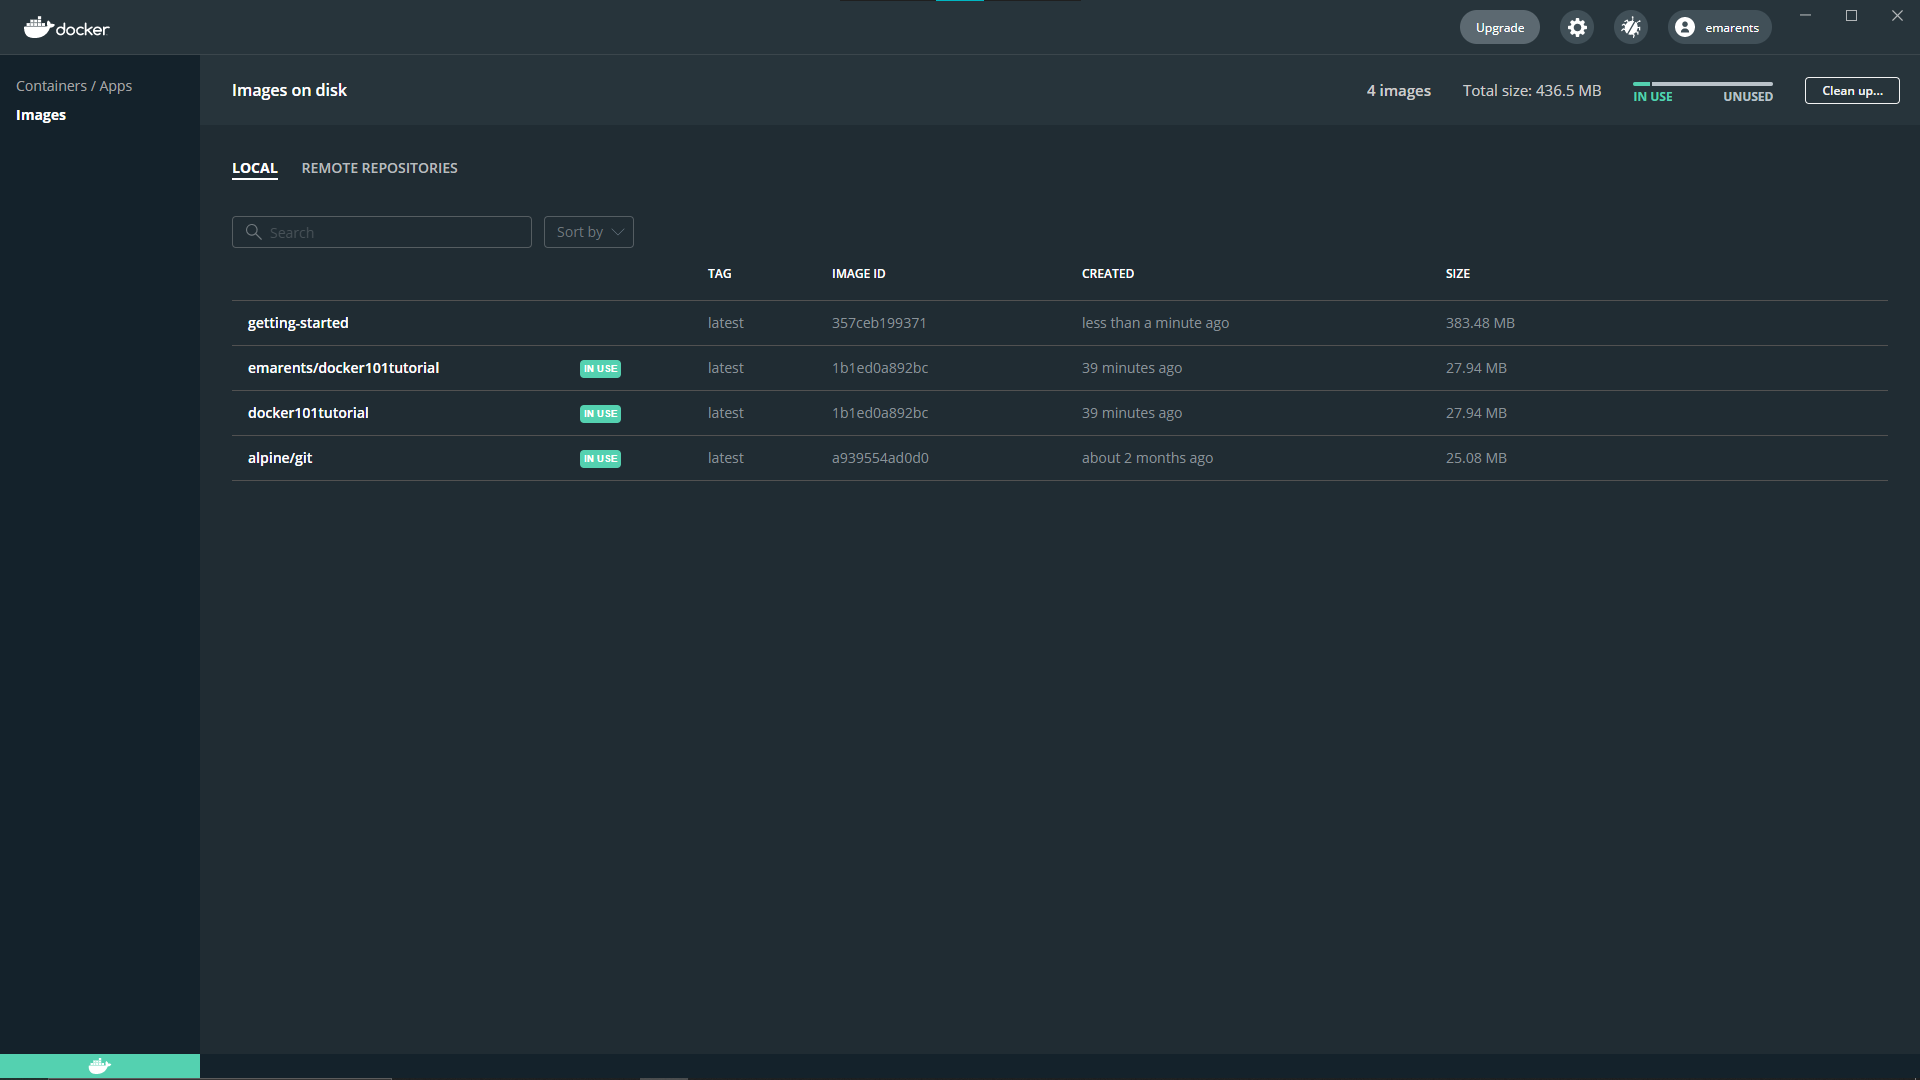
\includegraphics[width=\linewidth]{img/dockerImg.png}
    \label{fig:Dockerdesktop}
    \caption[De Docker desktop applicatie]{De Docker desktop applicatie, dit deel toont alle lokaal bewaarde images}
    \centering
\end{figure}
\begin{figure}[h]
    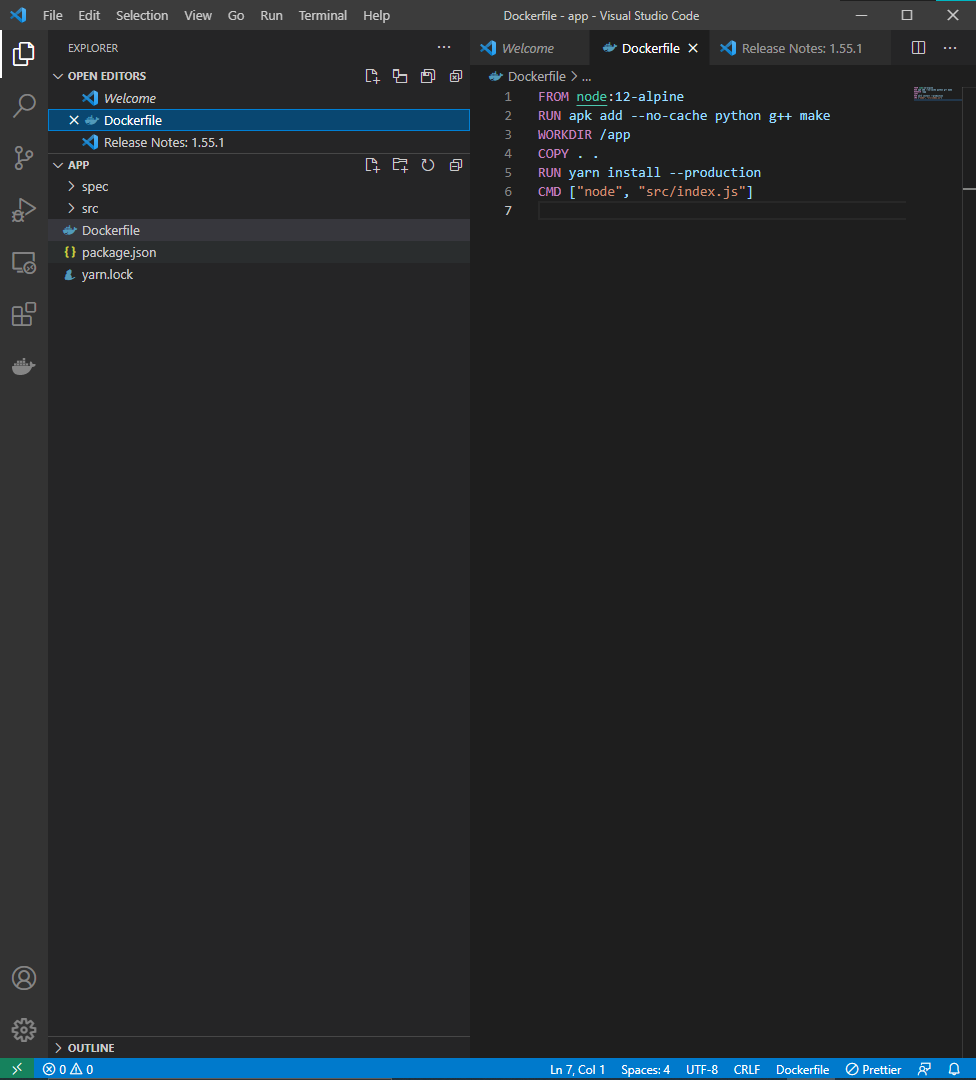
\includegraphics[width=\linewidth]{img/dockerSample.png}
    \label{fig:dockerfilevscode}
    \caption[Een dockerfile in VS code]{de dockerfile om een container  te creëren op basis van een node app, getoond in Visual Studio code}
    \centering
\end{figure}


Om ook compose en het verbinden van containers te demonstreren werd de data die demonstratie applicatie gebruikt ook een s weggeschreven naar een MySQL databank die in een eigen container draait. Eerst werd dit gedaan door een door Docker aangeboden container te gebruiken om zo een verkenning te doen van het netwerk waarop je Docker instantie staat. Met deze verkenner is het mogelijk om de juiste verbinding tussen de demo app en een mysql databank te leggen. Omdat het manueel verbinden moeilijk kan zijn werd ook Docker compose uitgelegd. Met een YAML-file kan je nodige containers definiëren en confituren dat bij het oproepen van composer ze samen opgestart worden en onmiddellijk verbonden zijn. Deze gebundelde containers worden ook samen getoond in de interface van de desktop applicatie.


\paragraph{Ervaring}
Docker’s gebruik is eenvoudig en is ook veel over te vinden online bij eventuele problemen.  De dokker desktop geeft een grafische interface voor het beheren van draaiende containers en images, maar dit is ook allemaal mogelijk via CLI. Met de voorwaarde hier dat bij het overnemen van commando’s deze soms over meerdere regels gespreid zijn en dus dat de commando prompt van Windows niet voldoende is en overgeschakeld moet worden naar powershell.  De desktop interface maakt het wel gemakkelijk om te beheren of dat je lokale Docker instantie draait waardoor het perfect mogelijk is om het geïnstalleerd te hebben staan en buiten gebruik niet door beïnvloed worden. Het starten en stoppen van Docker in een Linux omgeving is te doen via het proces beheer van Linux zelf.  De configuratie bestanden voor containers zijn geschreven in YAML en Visual studio code heeft zelf extensie om specifiek de Docker bestanden te ondersteunen.

\subsection{Fedora Podman}
Dit werd uitgevoerd in een VM met 4 GB ram en 20 gb harde schijfruimte
\paragraph{Installatie en set-up}
Bij de verse installatie van een Fedora workstation versie 53 was Podman al inbegrepen en was er geen nood om hem te installeren.

\paragraph{Ingebruikname}
Het reproduceren van de stappen van de Docker tutorial lukte eerst goed.  Het pullen, builden of draaien van images lukt analoog als met de Docker engine. Inclusief het gebruiken van dezelfde bestanden voor het definiëren van een container vooraleer deze te builden.  Bij het persisteren met volumes is ook geen verschil.
\begin{figure}[h]
    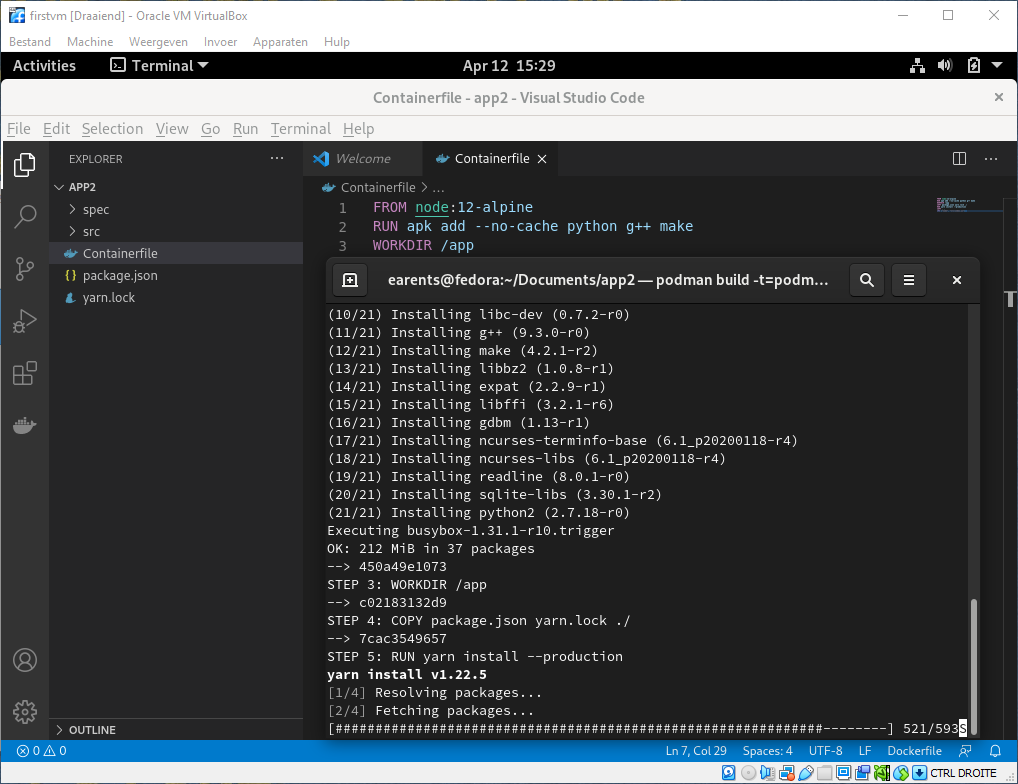
\includegraphics[width=\linewidth]{img/podmanbuild.png}
    \label{fig:podmanbuild}
    \caption[Een dockerfile in VS code om met podman te builden]{Hier maakt Podman met het inhoudelijk zelfde docker-/containerfile as Docker een image}
    \centering
\end{figure}
\begin{figure}[h]
    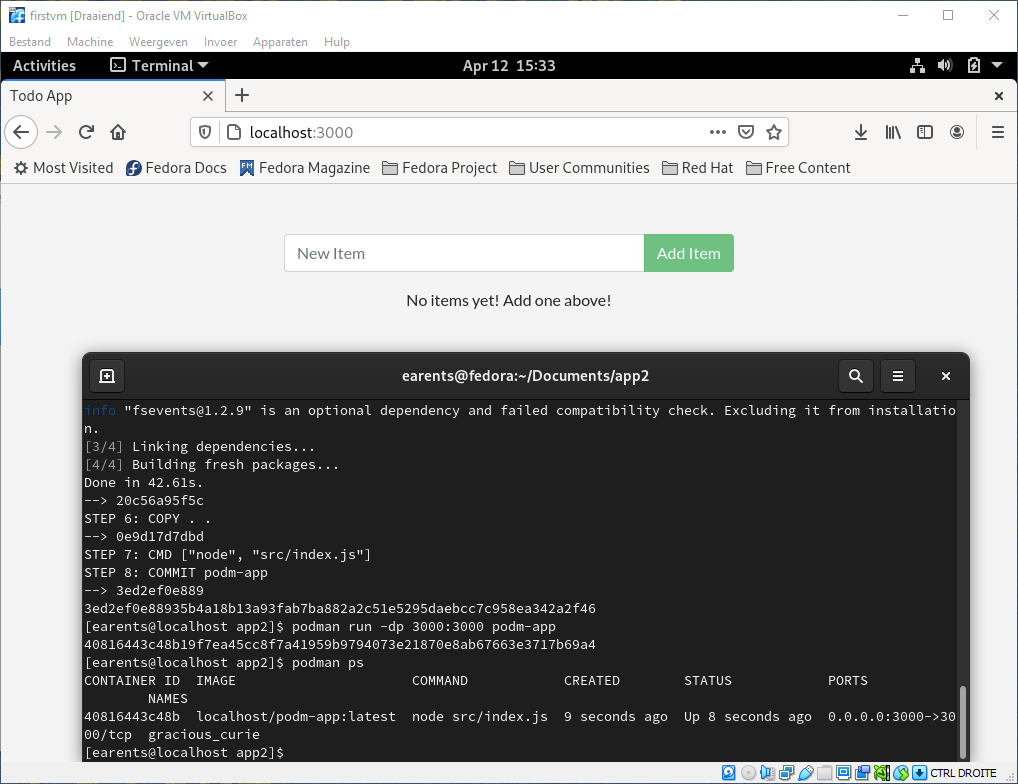
\includegraphics[width=\linewidth]{img/podmanrun.png}
    \label{fig:podmanrun}
    \caption[Podman die een web ap uitvoert]{hier is via command line de aangemaakte container gestart en wort deze op de achtergrond getoont in een webbrowser}
    \centering
\end{figure}

Bij Podman was het lokaal verbinden moeilijker. Het werken met Podman ingebouwde pods is minder goed uitgelegd dan het werken met Docker en het manueel verbinden.  Er bestaat ook een project om Docker compose na te bootsen voor Podman genaamd Podman Compose\footnote{\url{https://GitHub.com/containers/Podman-compose}} .  Hiermee kan je ook onmiddellijk meerdere containers samen laten bundelen en draaien, echter ook hier is het werken met de pod om de juiste poorten te zetten om te kunnen zien of dat het werkt een probleem.

\paragraph{Ervaring}
Het werken met Docker en Podman voor eenvoudige containers te draaien lijkt sterk op elkaar, veel commando’s zijn hetzelfde en geven ook een gelijkaardig resultaat. Doordat het standaard met Fedora gebundeld is was de installatie geen probleem. Ook moet voor het te kunnen gebruiker niet zelf de lokale Podman runtime starten vooraleer je deze kan gebruiken. Echter het werken met de pods van Podman is moeilijker dan met de eenvoudige verbinding die je met Docker kan leggen.

\subsection{Ubuntu Podman}
Dit werd uitgevoerd op een VM met 4gb ram en 30 GB geheugen ruimte. Initieel was die intentie om ook hier Podman een op uit te oefenen.

\paragraph{Installatie en set-up}
Na een basis installatie van Ubuntu LTS 20.4 is er initieel geprobeerd om een installatie te doen van Podman. Volgens de help pagina’s van Podman is het mogelijk op Podman te draaien op Ubuntu. Bij het instaleren op de manieren uitgelegd is er nooit succesvol een installatie gebeurt. Na een tijd tevergeefs te zoeken naar oorzaken is er overschakelt naar het uitproberen van een ander alternatief, namelijk Containerd.
Door lokaal Golang te hebben moet het mogelijk zijn om via Containerd te werken voor container runtime. Ook hier voor het effectief installeren van Golang ondervond ik problemen.  Eens Golang geïnstalleerd lukte het echter niet om Containerd uit te voeren

\paragraph{Ervaring}
Het is dus niet gelukt om zowel Podman als Containerd uit te voeren op Ubuntu. Voor het installeren van Podman kan het probleem zijn dat ten tijde van het proberen de repositories die Ubuntu aanreikte niet voorzien van de nodige bestanden. Voor Containerd zal het probleem liggen tussen gelijkaardige installatie problemen voor Golang. Dit gekoppeld met dat ik geen ervaring heb met Go heeft ervoor gezorgd dat ook Containerd niet lukte om uit te voeren.

\subsection{Kubernetes gebundeld met Docker desktop}
Dit werd opnieuw uitgevoerd aan de hand van de desktop installatie direct op de laptop. Voor de effectieve uitvoering van Kubernetes werd er gekeken naar het gebruik van GitHub als repository voor images.
\paragraph{Installatie en set-up}
Een volwaardige instantie van Kubernetes is gebundeld met de Docker desktop applicatie. Dit betekent wel dat het op Linux systemen niet gelijkaardig zal zijn.
Voor de GitHub Container Registry is het ten tijde van dit onderzoek nodig om manueel deel te nemen aan de beta versie. Ook stelt GitHub voor om een access token te maken voor het inloggen en verbinden met je container registry.

\paragraph{Ingebruikname}
Het weken met de GitHub container registry lukte vlot. Er zijn twee stappen die je moet doen vooraleer je kan pushen naar je registry. Met je access token kan je via de command line van Docker inloggen op het domein van de GitHub container registry Ghcr.io. Om dan effectief te pushen moet je nog wat aanpassen om lokaal duidelijk te maken dat je naar Ghr.io, om dit te doen moet de lokale container getagd worden en verwijzen naar de ghcr.io/username/containername vooraleer je deze kan pushen. Deze expliciete verwijzing is nodig want Docker zal standaard altijd de Docker hub gebruiken al remote locatie. Het pullen van images van de container registry gebeurt door manueel te specifiëren dat er van daar moet worden gepulled om zo het niet op Dockers hub te zoeken.

De gebundelde Kubernetes van de Docker desktop lukte niet om te gebruiken. Bij het opstarten van Kubernetes via de desktop worden alle nodige onderdelen geïmporteerd en opgestart in hun eigen containers. Kubernetes is niet volledig kunnen starten. Windows task manager gaf aan dat de laptops processor en ram geheugen overbelast werden. Verder toonde de interface van Docker desktop hoe bepaalde containers voor de werking opstartte, afgebroken werden en weer opgestart werden.

\paragraph{Ervaring}
Het werken met de GitHub Container Registry loopt vlot het voornaamste jammerlijke is dat zelfs als je inlogt op de registry dat Docker altijd nog eerst zal proberen met de Docker hub.
Zoals aangegeven lukte Kubernetes niet. Dit zal voornamelijk liggen aan de verouderde laptop die gebruikt werd, gecombineerd met dat de Kubernetes instantie veel eist. De laptop voldoet aan de minimumvereisten volgen de Docker help pagina’s maar mogelijk zijn niet van toepassing op de inbegrepen Kubernetes.  


\subsection{Podman met Minikube voor Kubernetes}
In een Fedora workstation 53 VM met 4 GB ram, twee virtuele CPU’s en 32 GB harde schijfruimte Ook werd er eerst geoefend om te zien of Podman met de GitHub Container Registry kan werken.
\paragraph{Installatie en set-up}
Voor de VM kwam er wat extra set up bij wan Minikube vraagt voor minstens 20 gigabyte vrij en 2 processoren.
Minikube raad ook aan om Cri-o te hebben om Podman te gebruiken als engine in plaats van Docker. Dus dit werd ook geïnstalleerd, op basis van cri-o help pagina’s.  Ook werd Minikube zelf geïnstalleerd.

\paragraph{Ingebruikname}
Het werken met de GitHub container registry in Podman is volledig analoog met de werking in Docker. Podman zoek ook standaard eerst op Docker hub dus moet er manueel gespecificeerd worden dat je een ander registry wilt gebruiken. Tijdens het werken met Podman en GitHub werd er ook een recent gepubliceerd blog van de Fedora Magazine die eens overloopt hoe je met Podman minder grote container images kan maken. Door in het Dockerfile of container file voor je container image optionele dependencies en feature die standaard in je base image staan te verwijderen kan je image grootte verkleind worden. De blog gaf ook een voorbeeld voor het werken met Buildah voor het maken van een image zonder een base image te hebben, maar installatie van Buildah lukte niet.

De ondersteuning die Minikube heeft voor Podman op het moment van dit onderzoek in nog steeds in een experimentele fase. Bij een eerste keer proberen starten van Minikube met Podman en Cri-o voor driver en effectieve runtime kwam er een gekende fout. Het oplossen van deze fout die eigen is aan Podman wordt uitgelegd op de Minikube help pagina’s voor Podman\footnote{\url{https://minikube.sigs.k8s.io/docs/drivers/Podman/}} . Door de fout op te lossen kan Minikube, en alle emoticons die het gebruikt, gestart worden.

Eens Minikube opgestart kan met een lokale instantie van Kubernetes gewerkt worden. Minikube komt met de command line interface voor Kubernetes. Zo is het mogelijk om aan Minikube doorgegeven welke kubectl commando’s moeten worden uitgevoerd. Het is echter ook mogelijk om individueel kubectl te installeren, Minikube zal bij het opstarten er zelf voor zorgen dat deze lokale installatie uitgevoerd wordt op de cluster die Minikube beheerd.  Minikube commando’s staan in voor het beheren van de cluster in zijn geheel zoals het starten stoppen of blootstellen van containers naar buiten. Kubectl is de tool om te werken binnen de cluster en met de containers erin.
\begin{figure}[h]
    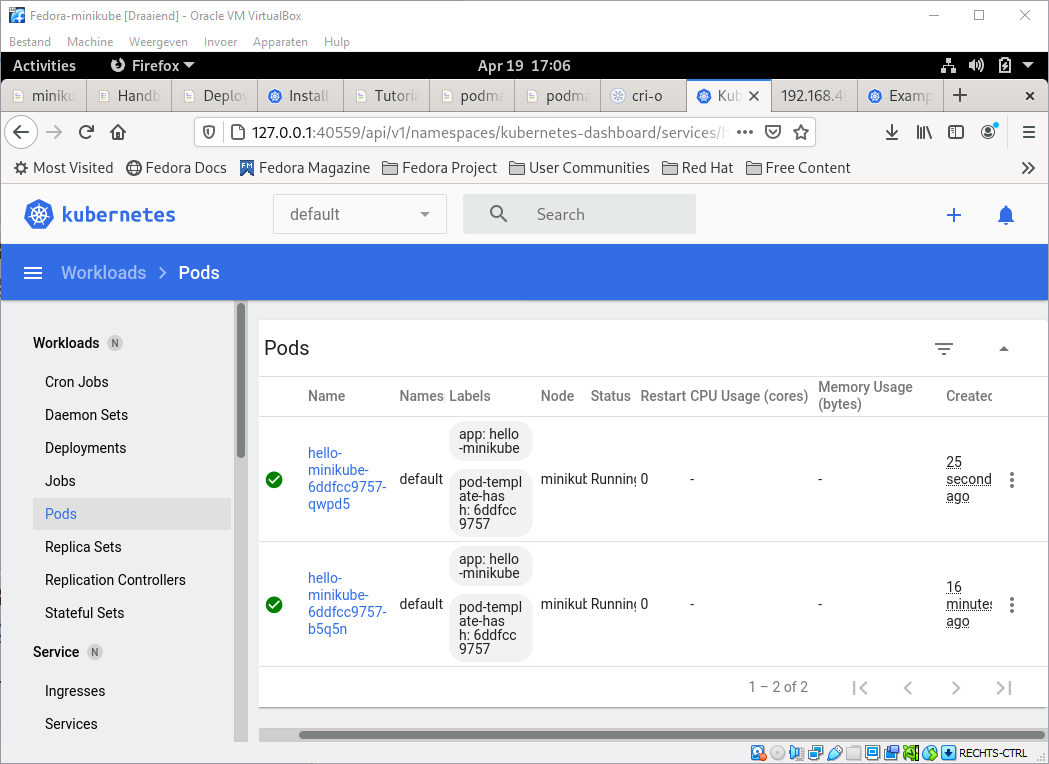
\includegraphics[width=\linewidth]{img/kubenetesDash.png}
    \label{fig:kubenetesDash}
    \caption[the kubenetes Dashboard]{hier toont de Kubernetes dashboard dat een nieuwe pod van de hellominikube container recent gestart is}
    \centering
\end{figure}

Met de lokale Kubernetes instantie is het verder gelukt om Kubernetes uit te proberen. Op basis van een standaardvoorbeeld voor Wordpress en MySQL\footnote{\url{https://kubernetes.io/docs/tutorials/stateful-application/mysql-wordpress-persistent-volume/}}  lukt het om snel de nodige Kustomization.yaml file aan te maken een door te geven aan Kubernetes via kubectl. Het openzetten naar buiten toe gaat dan via Minikube. Verder laat Minikube je ook toe om vlug de browser gebaseerde dashboard van je lokale instantie te openen. Hiermee kan je veel van de functionaliteiten van Kubernetes ook doen. Inclusief een publieke image van de GitHub container registry via deze interface pullen en onmiddellijk starten. Kubernetes heeft echter geen voor de hand liggende methode om lokaal bewaarde images of private images te gebruiken bij het starten van een container.

\paragraph{Ervaring}
Podman met GitHub container registry was zeer makkelijk en was zoals vermeld volledig analoog aan de Docker methode. De blogpost gaf een korte uitleg over hoe een container file verder aangepast kan worden om bepaalde zaken te configureren. Jammer genoeg lukte Buildah niet door een conflict tijdens de installatie met de al geïnstalleerde Podman. Buildah zou ook enkel nodig zijn ov vanaf nul een nieuwe image te maken en het juist kunnen werken met een vertrekpunt voor images acht ik belangrijker dus is Podman’s build voldoende.

Het starten van Minikube met Podman vergt wat meer configuratie maar is niet onredelijk. Het gebruikt veel emoticons om berichten te accentueren wat afhankelijk van persoonlijke smaak een minpunt kan zijn. Eens de Minikube Kubernetes gestart is merk je niet meer waarop het effectief draait. Ook is Minikube licht genoeg om zonder problemen te werken met 4 GB ram, iets wat de Docker desktop Kubernetes niet kon.

Kubernetes zelf is zeer goed. Er zijn veel voorbeelden voor te vinden en werkt binnen Minikube. De Dashboard van Kubernetes is ook een zeer grote pluspunt. Het laat een gebruiker toe om de volledige cluster te beheren zonder noodzakelijk via de commandolijn te werken. Ook toont het bij het kiezen van een actie met het dashboard wat de equivalente commando zou zijn om het via command line te doen.


\subsection{Docker engine voor Nomad}
Hiervoor weer de Ubuntu deels om te zien of dat het installeren van Docker zou lukken en omdat deze verder al aan alle eisen voor Nomad voldeed.
\paragraph{Installatie en set-up}
De Docker engine installeren en opstarten lukt zonder problemen. Ook het installeren van Nomad zelf gaf geen complicaties.
\paragraph{Ingebruikname}
Na het installeren van de Docker engine werd er eerst getest of dat alles  werkte zoals het direct op de laptop lukte. Hierbij werden geen problemen ondervonden. Hierna werd een dev omgeving Nomad instantie opgestart om eens mee te werken.
\begin{figure}[h]
    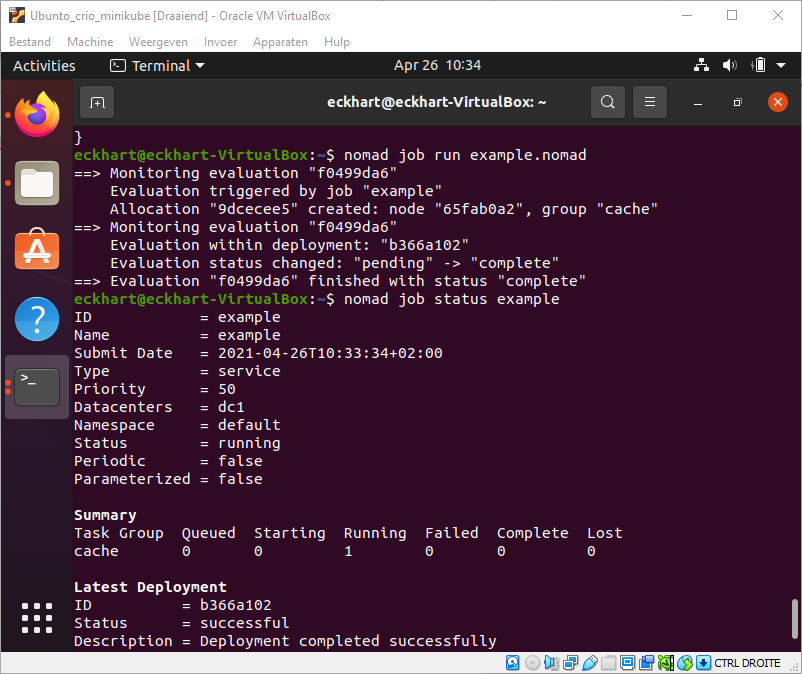
\includegraphics[width=\linewidth]{img/nomadrun.png}
    \label{fig:nomadrun}
    \caption[Een voorbeeld Nomad job]{hier wordt via de cli van Nomad de example.nomad job gestart}
    \centering
\end{figure}
\begin{figure}[h]
    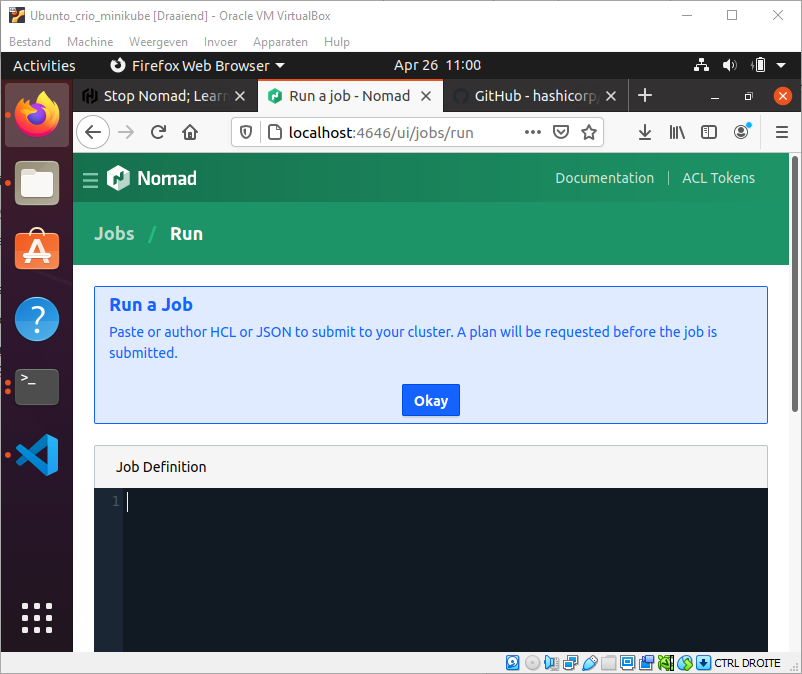
\includegraphics[width=\linewidth]{img/nomdaddash.png}
    \label{fig:nomdaddash}
    \caption[de nomad dashboard]{de dashboard weergave om een job te starten met Nomad}
    \centering
\end{figure}

Hashi Corp heeft een korte tutorial\footnote{\url{https://learn.hashicorp.com/collections/nomad/get-started}} die een inleiding geeft tot het werken met Nomad. Het legt uit wat de workflow is een geeft een voorbeeld toegepast op een kleine container image.  Hier wordt hun eigen .nomad bestandsindeling eens aangehaald die gebruikt wordt voor het configureer van de “jobs” of taken die Nomad moet uitvoeren. Om Nomad iets te laten doen moet eerst een job bestand gemaakt worden. Deze moet vervolgens via command line of de web interface ingepland worden en vervolgens nog eens afzonderlijk uitgevoerd worden. Een enkele container draaien en dupliceren lukte maar het achterhalen hoe een Wordpress site te draaien lukte niet.

\paragraph{Ervaring}
Door Nomad werking met jobs voor alle taken is er een duidelijk verschil met Kubernetes. Een groot voordeel is dat Nomad meer kan beheren dan enkel containers. Maar het heeft zeker zijn minpunten. Zo is de eigen markup voor de configuratie een bijkomende barrière voor het werken met Nomad in vergelijking met de al veelgebruikte YAML die Docker, Podman en Kubernetes allemaal gebruiken.  Visual studio code heeft gelukkig een extensie voor de Configuratie Taal die hashicorp gebruikt die het werken met deze .Nomad  bestanden helpt. Nomad heeft ook een web browser gebaseerde interface maar deze toont niet wat een equivalent commando voor de command line zou zijn. Het is ook in het algemeen minder gebruikt dan Kubernetes waardoor uitleg en integratie minder is.  

\section{Samengevatte resultaten software Tests}
%% TODO: insert table comarisons?
Dit deel vergelijkt samengevat eens de technologieën die gebruikt zijn. Enkel voor orchestration is er een duidelijke voorkeur voor Kubernetes als leermiddel.

\subsection{Runtimes}

In basis gebruik lijken Docker en Podman goed op elkaar. De grootste verschillen zitten in de installatie en de eigen werking voor meerdere samenhangende containers. Qua installatie komt Podman standaard geïnstalleerd in Fedora, en moet Docker altijd geïnstalleerd worden. De Docker compose die afhankelijk afzonderlijk geïnstalleerd moet worden maakt het verbinden van container mogelijk  Het equivalent in Podman met de pods is iets complexer en zelfs met een extra overbrugging van Podman Compose niet voor de hand liggend. Echter deze verbinding tussen container kan ook gedaan worden in Kubernetes en is bij gebruik van Kubernetes niet meer zo belangrijk.

Verder is de Docker desktop voor het leren maar een kleine meerwaarde. Het is ten eerste niet beschikbaar op linux systemen. Ten tweede moeten veel functionaliteiten nog via de command line uitgevoerd worden. De desktop applicatie een overzicht van lokale images het maken van een nieuwe image moet via command line interface. Ten derde is de gebundelde Kubernetes zwaarder dan een Kubernetes instantie met Minikube.

\subsection{Repositories}

Tussen de twee gebruikte repository is er niet meteen een de beter is dan de andere. De Docker hub wordt door zowel Docker als Podman gebruikt als standaard doel om image te pushen. Dit beteken dat er weinig aangepast moet worden om effectief te pushen of pullen. Echter de Docker hub zet standaard images publiek en heeft maar een private image mogelijkheid voor gratis accounts. De GitHub container registry daarentegen zou een beetje extra werk vragen om het doel voor het pushen van een image te selecteren. Het zou wel geen extra account nodigen hebben als de student al reeds met GitHub werkt. Over de specifieke kosten en regeling van de GitHub container registry kan er nog geen uitspraak gedaan worden doordat deze nog in bèta fase is. Zou het zelfde limiet  van 500 mb voor private containers gelden als op de rest van GitHub packages zou deze te klein zijn om meer te beteken dan één of enkele private images.

\subsection{Orchestration}

Voor orchestration is Kubernetes de beste van de twee geteste voor het werken met containers. Zo heeft het een dashboard weergave die niet alleen de noodzaak voor het werken via command line minimaliseert, het toont ook bij het uitvoeren van taken via deze dasboard de equivalente commando’s om het via cli te doen. Om met Kubernetes te leren werken is de beschikbaarheid Minikube ook een pluspunt. Minikube helpt om een lokale Kubernetes cluster op te starten en beheren. Verder kan Minikube ook de juiste verbindingen maken om een keuze aan achterliggende runtime te hebben.  Minikube heeft de beste ondersteuning voor Docker als engine maar kan met wat extra configuratie een het installeren kan Cri-o als hulpstuk ook met Podman als runtime werken. één van de grotere minpunten die eigen is aan Kubernetes is dat het moeilijk is om containers te draaien op basis van lokaal bewaarde images of privé bewaard in een repository.

Om specifiek met containers te werken is Nomad minder aan te raden. De hasicorp configuration language is ook een extra stap in het leerproces. Het kan dat een student Yaml dei Kubernetes gebruikt nog niet gezien heeft, maar de kans is groter dat de student ook Yaml elders zal tegenkomen dan de Hasicorp markup. Ook iets dat het leren ten nadele zou komen ten opzichte van Kubernetes is dat de dashboard niet de equivalente commando’s toont, dit is deels toe te kennen aan de methodologie van Nomad om aanpassingen aan je draaiende containers te doen op basis van jobs, die telkens geschreven moeten worden in de hasicorp configuration language.
